%********************************************************************
% Appendix
%*******************************************************
% If problems with the headers: get headings in appendix etc. right
%\markboth{\spacedlowsmallcaps{Appendix}}{\spacedlowsmallcaps{Appendix}}

%********************************************************************
% TTL Reference
%********************************************************************
\chapter{TTL Reference}

\LE includes a number of \ac{TTL} \acp{IC}. These are pre-packaged digital logic circuits that perform specific, well-defined functions. There are, literally, hundreds of \ac{TTL} \acp{IC} available for purchase from electronics warehouses but \LE includes only $ 35 $ of the most commonly-used devices. Figure \ref{fig:50-74HC595} shows three surface-mounted \acp{IC} on a circuit board.

\begin{figure}[H]
	\centering
	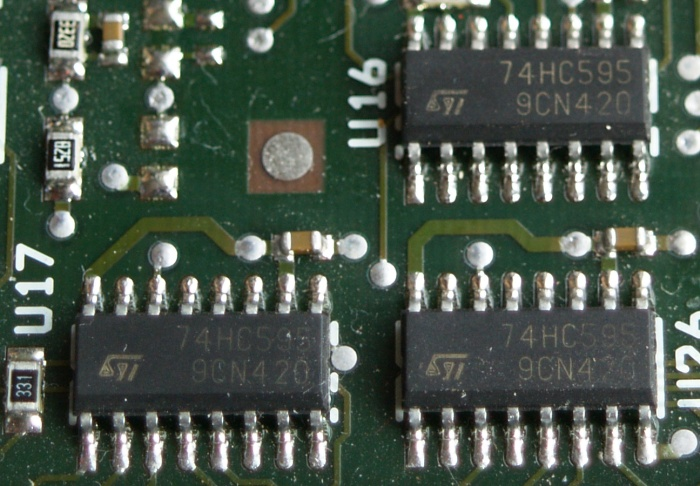
\includegraphics[width=\maxwidth{.75\linewidth}]{gfx/50-74HC595}
	\caption{Three Surface-Mounted Integrated Circuits}
	\label{fig:50-74HC595}
\end{figure}

\section{7400: Quad 2-Input NAND Gate}

This device contains four independent 2-input NAND gates. Figure \ref{fig:50-7400} is a logic diagram of one of the four circuits.

\begin{figure}[H]
	\centering
	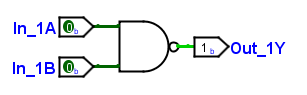
\includegraphics{gfx/50-7400}
	\caption{7400: Single NAND Gate Circuit}
	\label{fig:50-7400}
\end{figure}

The 7400 device in \LE uses the wiring connections indicated in Table \ref{tab:50-7400}.

\begin{table}[H]
	\sffamily
	\newcommand{\head}[1]{\textcolor{white}{\textbf{#1}}}		
	\begin{center}
		\rowcolors{2}{gray!10}{white} % Color every other line a light gray
		\begin{tabular}{rl} 
			\rowcolor{black!75}
			\head{Logisim Label} & \head{Function} \\
			Input: 1   & In 1A  \\
			Input: 2   & In 1B  \\
			Output: 3  & Out 1Y \\
			Input: 4   & In 2A  \\
			Input: 5   & In 2B  \\
			Output: 6  & Out 2Y \\
			Output: 8  & Out 3Y \\
			Input: 9   & In 3A  \\
			Input: 10  & In 3B  \\
			Output: 11 & Out 4Y \\
			Input: 12  & In 4A  \\
			Input: 13  & In 4B  \\
		\end{tabular}
	\end{center}
	\caption{Pinout For 7400}
	\label{tab:50-7400}
\end{table}

\section{7402: Quad 2-Input NOR Gate}

This device contains four independent 2-input NOR gates. Figure \ref{fig:50-7402} is a logic diagram of one of the four circuits.

\begin{figure}[H]
	\centering
	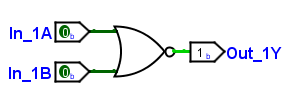
\includegraphics{gfx/50-7402}
	\caption{7402: Single NOR Gate Circuit}
	\label{fig:50-7402}
\end{figure}

The 7402 device in \LE uses the wiring connections indicated in Table \ref{tab:50-7402}.

\begin{table}[H]
	\sffamily
	\newcommand{\head}[1]{\textcolor{white}{\textbf{#1}}}		
	\begin{center}
		\rowcolors{2}{gray!10}{white} % Color every other line a light gray
		\begin{tabular}{rl} 
			\rowcolor{black!75}
			\head{Logisim Label} & \head{Function} \\
			Input: 1   & In 1A  \\
			Input: 2   & In 1B  \\
			Output: 3  & Out 1Y \\
			Input: 4   & In 2A  \\
			Input: 5   & In 2B  \\
			Output: 6  & Out 2Y \\
			Output: 8  & Out 3Y \\
			Input: 9   & In 3A  \\
			Input: 10  & In 3B  \\
			Output: 11 & Out 4Y \\
			Input: 12  & In 4A  \\
			Input: 13  & In 4B  \\
		\end{tabular}
	\end{center}
	\caption{Pinout For 7402}
	\label{tab:50-7402}
\end{table}

\section{7404: Hex Inverter}

This device contains six independent inverters. Figure \ref{fig:50-7404} is a logic diagram of one of the six circuits.

\begin{figure}[H]
	\centering
	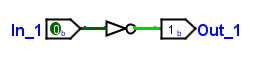
\includegraphics{gfx/50-7404}
	\caption{7404: Single Inverter Circuit}
	\label{fig:50-7404}
\end{figure}

The 7404 device in \LE uses the wiring connections indicated in Table \ref{tab:50-7404}.

\begin{table}[H]
	\sffamily
	\newcommand{\head}[1]{\textcolor{white}{\textbf{#1}}}		
	\begin{center}
		\rowcolors{2}{gray!10}{white} % Color every other line a light gray
		\begin{tabular}{rl} 
			\rowcolor{black!75}
			\head{Logisim Label} & \head{Function} \\
			Input: 1   & In 1  \\
			Output: 2  & Out 1  \\
			Input: 3   & In 2 \\
			Output: 4  & Out 2  \\
			Input: 5   & In 3  \\
			Output: 6  & Out 3 \\
			Output: 8  & Out 4  \\
			Input: 9   & In 4  \\
			Output: 10 & Out 5  \\
			Input: 11  & In 5  \\
			Output: 12 & Out 6 \\
			Input: 13  & In 6  \\
		\end{tabular}
	\end{center}
	\caption{Pinout For 7404}
	\label{tab:50-7404}
\end{table}

\section{7408: Quad 2-Input AND Gate}

This device contains four independent 2-input AND gates. Figure \ref{fig:50-7408} is a logic diagram of one of the four circuits.

\begin{figure}[H]
	\centering
	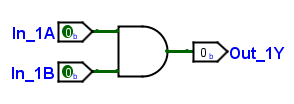
\includegraphics{gfx/50-7408}
	\caption{7408: Single AND Gate Circuit}
	\label{fig:50-7408}
\end{figure}

The 7408 device in \LE uses the wiring connections indicated in Table \ref{tab:50-7408}.

\begin{table}[H]
	\sffamily
	\newcommand{\head}[1]{\textcolor{white}{\textbf{#1}}}		
	\begin{center}
		\rowcolors{2}{gray!10}{white} % Color every other line a light gray
		\begin{tabular}{rl} 
			\rowcolor{black!75}
			\head{Logisim Label} & \head{Function} \\
			Input: 1   & In 1A  \\
			Input: 2   & In 1B  \\
			Output: 3  & Out 1Y \\
			Input: 4   & In 2A  \\
			Input: 5   & In 2B  \\
			Output: 6  & Out 2Y \\
			Output: 8  & Out 3Y \\
			Input: 9   & In 3A  \\
			Input: 10  & In 3B  \\
			Output: 11 & Out 4Y \\
			Input: 12  & In 4A  \\
			Input: 13  & In 4B  \\
		\end{tabular}
	\end{center}
	\caption{Pinout For 7408}
	\label{tab:50-7408}
\end{table}

\section{7410: Triple 3-Input NAND Gate}

This device contains three independent 3-input NAND gates. Figure \ref{fig:50-7410} is a logic diagram of one of the three circuits.

\begin{figure}[H]
	\centering
	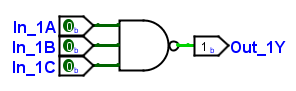
\includegraphics{gfx/50-7410}
	\caption{7410: Single 3-Input NAND Gate Circuit}
	\label{fig:50-7410}
\end{figure}

The 7410 device in \LE uses the wiring connections indicated in Table \ref{tab:50-7410}.

\begin{table}[H]
	\sffamily
	\newcommand{\head}[1]{\textcolor{white}{\textbf{#1}}}		
	\begin{center}
		\rowcolors{2}{gray!10}{white} % Color every other line a light gray
		\begin{tabular}{rl} 
			\rowcolor{black!75}
			\head{Logisim Label} & \head{Function} \\
			Input: 1   & In 1A  \\
			Input: 2   & In 1B  \\
			Input: 3   & In 2A \\
			Input: 4   & In 2B  \\
			Input: 5   & In 2C  \\
			Output: 6  & Out 2Y \\
			Output: 8  & Out 3Y \\
			Input: 9   & In 3A  \\
			Input: 10  & In 3B  \\
			Input: 11  & In 3C \\
			Output: 12 & Out 1Y  \\
			Input: 13  & In 1C  \\
		\end{tabular}
	\end{center}
	\caption{Pinout For 7410}
	\label{tab:50-7410}
\end{table}

\section{7411: Triple 3-Input AND Gate}

This device contains three independent 3-input AND gates. Figure \ref{fig:50-7411} is a logic diagram of one of the three circuits.

\begin{figure}[H]
	\centering
	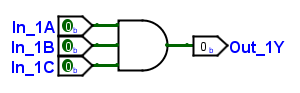
\includegraphics{gfx/50-7411}
	\caption{7411: Single 3-Input AND Gate Circuit}
	\label{fig:50-7411}
\end{figure}

The 7411 device in \LE uses the wiring connections indicated in Table \ref{tab:50-7411}.

\begin{table}[H]
	\sffamily
	\newcommand{\head}[1]{\textcolor{white}{\textbf{#1}}}		
	\begin{center}
		\rowcolors{2}{gray!10}{white} % Color every other line a light gray
		\begin{tabular}{rl} 
			\rowcolor{black!75}
			\head{Logisim Label} & \head{Function} \\
			Input: 1   & In 1A  \\
			Input: 2   & In 1B  \\
			Input: 3   & In 2A \\
			Input: 4   & In 2B  \\
			Input: 5   & In 2C  \\
			Output: 6  & Out 2Y \\
			Output: 8  & Out 3Y \\
			Input: 9   & In 3A  \\
			Input: 10  & In 3B  \\
			Input: 11  & In 3C \\
			Output: 12 & Out 1Y  \\
			Input: 13  & In 1C  \\
		\end{tabular}
	\end{center}
	\caption{Pinout For 7411}
	\label{tab:50-7411}
\end{table}

\section{7413: Dual 4-Input NAND Gate (Schmitt-Trigger)}

This device contains two independent 4-input NAND gates. Schmitt-triggers are a special type of device that are used to filter out spurious noise on a circuit. They are designed to change from low-to-high or high-to-low only when the input voltage reaches a preset level but not if the voltage randomly fluctuates without crossing the set-points. This device is essentially the same as the 7418. Figure \ref{fig:50-7413} is a logic diagram of one of the two circuits.

\begin{figure}[H]
	\centering
	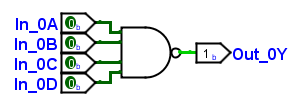
\includegraphics{gfx/50-7413}
	\caption{7413: Single 4-Input NAND Gate Circuit}
	\label{fig:50-7413}
\end{figure}

The 7413 device in \LE uses the wiring connections indicated in Table \ref{tab:50-7413}.

\begin{table}[H]
	\sffamily
	\newcommand{\head}[1]{\textcolor{white}{\textbf{#1}}}		
	\begin{center}
		\rowcolors{2}{gray!10}{white} % Color every other line a light gray
		\begin{tabular}{rl} 
			\rowcolor{black!75}
			\head{Logisim Label} & \head{Function} \\
			Input: 1    & In A0  \\
			Input: 2    & In B0  \\
			Pin 3: NC   & Not Connected \\
			Input: 4    & In C0  \\
			Input: 5    & In D0  \\
			Output: 6   & Out Y0 \\
			Output: 8   & Out Y1 \\
			Input: 9    & In D1  \\
			Input: 10   & In C1  \\
			Pin 11: NC  & Not Connected \\
			Input: 12   & In B1  \\
			Input: 13    & In A1  \\
		\end{tabular}
	\end{center}
	\caption{Pinout For 7413}
	\label{tab:50-7413}
\end{table}

\section{7414: Hex Inverter (Schmitt-Trigger)}

This device contains six independent inverters. Schmitt-triggers are a special type of device that are used to filter out spurious noise on a circuit. They are designed to change from low-to-high or high-to-low only when the input voltage reaches a preset level but not if the voltage randomly fluctuates without crossing the set-points. This device is essentially the same as the 7419. Figure \ref{fig:50-7414} is a logic diagram of one of the six circuits.

\begin{figure}[H]
	\centering
	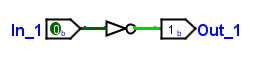
\includegraphics{gfx/50-7404}
	\caption{7414: Single Inverter Circuit}
	\label{fig:50-7414}
\end{figure}

The 7414 device in \LE uses the wiring connections indicated in Table \ref{tab:50-7414}.

\begin{table}[H]
	\sffamily
	\newcommand{\head}[1]{\textcolor{white}{\textbf{#1}}}		
	\begin{center}
		\rowcolors{2}{gray!10}{white} % Color every other line a light gray
		\begin{tabular}{rl} 
			\rowcolor{black!75}
			\head{Logisim Label} & \head{Function} \\
			Input: 1   & In 1  \\
			Output: 2  & Out 1  \\
			Input: 3   & In 2 \\
			Output: 4  & Out 2  \\
			Input: 5   & In 3  \\
			Output: 6  & Out 3 \\
			Output: 8  & Out 4  \\
			Input: 9   & In 4  \\
			Output: 10 & Out 5  \\
			Input: 11  & In 5  \\
			Output: 12 & Out 6 \\
			Input: 13  & In 6  \\
		\end{tabular}
	\end{center}
	\caption{Pinout For 7414}
	\label{tab:50-7414}
\end{table}

\section{7418: Dual 4-Input NAND Gate (Schmitt-Trigger Inputs)}

This device contains two independent 4-input NAND gates. Schmitt-triggers are a special type of device that are used to filter out spurious noise on a circuit. They are designed to change from low-to-high or high-to-low only when the input voltage reaches a preset level but not if the voltage randomly fluctuates without crossing the set-points. This device is essentially the same as the 7413. Figure \ref{fig:50-7418} is a logic diagram of one of the two circuits.

\begin{figure}[H]
	\centering
	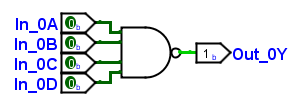
\includegraphics{gfx/50-7413}
	\caption{7418: Single 4-Input NAND Gate Circuit}
	\label{fig:50-7418}
\end{figure}

The 7418 device in \LE uses the wiring connections indicated in Table \ref{tab:50-7418}.

\begin{table}[H]
	\sffamily
	\newcommand{\head}[1]{\textcolor{white}{\textbf{#1}}}		
	\begin{center}
		\rowcolors{2}{gray!10}{white} % Color every other line a light gray
		\begin{tabular}{rl} 
			\rowcolor{black!75}
			\head{Logisim Label} & \head{Function} \\
			Input: 1   & In A0  \\
			Input: 2   & In B0  \\
			Pin 3 NC   & Not Connected \\
			Input: 4   & In C0  \\
			Input: 5   & In D0  \\
			Output: 6  & Out Y0 \\
			Output: 8  & Out Y1 \\
			Input: 9   & In D1  \\
			Input: 10  & In C1  \\
			Pin 11 NC  & Not Connected \\
			Input: 12 & In B1  \\
			Input: 13  & In A1  \\
		\end{tabular}
	\end{center}
	\caption{Pinout For 7418}
	\label{tab:50-7418}
\end{table}

\section{7419: Hex Inverter (Schmitt-Trigger)}

This device contains six independent inverters. Schmitt-triggers are a special type of device that are used to filter out spurious noise on a circuit. They are designed to change from low-to-high or high-to-low only when the input voltage reaches a preset level but not if the voltage randomly fluctuates without crossing the set-points. This device is essentially the same as the 7414. Figure \ref{fig:50-7419} is a logic diagram of one of the six circuits.

\begin{figure}[H]
	\centering
	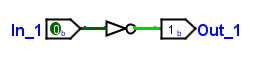
\includegraphics{gfx/50-7404}
	\caption{7419: Single Inverter Circuit}
	\label{fig:50-7419}
\end{figure}

The 7419 device in \LE uses the wiring connections indicated in Table \ref{tab:50-7419}.

\begin{table}[H]
	\sffamily
	\newcommand{\head}[1]{\textcolor{white}{\textbf{#1}}}		
	\begin{center}
		\rowcolors{2}{gray!10}{white} % Color every other line a light gray
		\begin{tabular}{rl} 
			\rowcolor{black!75}
			\head{Logisim Label} & \head{Function} \\
			Input: 1   & In 1  \\
			Output: 2  & Out 1  \\
			Input: 3   & In 2 \\
			Output: 4  & Out 2  \\
			Input: 5   & In 3  \\
			Output: 6  & Out 3 \\
			Output: 8  & Out 4  \\
			Input: 9   & In 4  \\
			Output: 10 & Out 5  \\
			Input: 11  & In 5  \\
			Output: 12 & Out 6 \\
			Input: 13  & In 6  \\
		\end{tabular}
	\end{center}
	\caption{Pinout For 7419}
	\label{tab:50-7419}
\end{table}

\section{7420: Dual 4-Input NAND Gate}

This device contains two independent 4-input NAND gates. Figure \ref{fig:50-7420} is a logic diagram of one of the two circuits.

\begin{figure}[H]
	\centering
	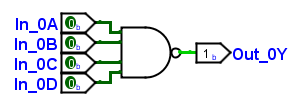
\includegraphics{gfx/50-7413}
	\caption{7420: Single 4-Input NAND Gate Circuit}
	\label{fig:50-7420}
\end{figure}

The 7420 device in \LE uses the wiring connections indicated in Table \ref{tab:50-7420}.

\begin{table}[H]
	\sffamily
	\newcommand{\head}[1]{\textcolor{white}{\textbf{#1}}}		
	\begin{center}
		\rowcolors{2}{gray!10}{white} % Color every other line a light gray
		\begin{tabular}{rl} 
			\rowcolor{black!75}
			\head{Logisim Label} & \head{Function} \\
			Input: 1   & In A0  \\
			Input: 2   & In B0  \\
			Pin 3 NC   & Not Connected \\
			Input: 4   & In C0  \\
			Input: 5   & In D0  \\
			Output: 6  & Out Y0 \\
			Output: 8  & Out Y1 \\
			Input: 9   & In D1  \\
			Input: 10  & In C1  \\
			Pin 11 NC  & Not Connected \\
			Input: 12 & In B1  \\
			Input: 13  & In A1  \\
		\end{tabular}
	\end{center}
	\caption{Pinout For 7420}
	\label{tab:50-7420}
\end{table}

\section{7421: Dual 4-Input AND Gate}

This device contains two independent 4-input AND gates. Figure \ref{fig:50-7421} is a logic diagram of one of the two circuits.

\begin{figure}[H]
	\centering
	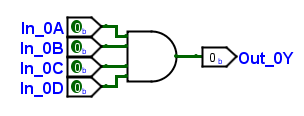
\includegraphics{gfx/50-7421}
	\caption{7421: Single 4-Input AND Gate Circuit}
	\label{fig:50-7421}
\end{figure}

The 7421 device in \LE uses the wiring connections indicated in Table \ref{tab:50-7421}.

\begin{table}[H]
	\sffamily
	\newcommand{\head}[1]{\textcolor{white}{\textbf{#1}}}		
	\begin{center}
		\rowcolors{2}{gray!10}{white} % Color every other line a light gray
		\begin{tabular}{rl} 
			\rowcolor{black!75}
			\head{Logisim Label} & \head{Function} \\
			Input: 1   & In A0  \\
			Input: 2   & In B0  \\
			Pin 3 NC   & Not Connected \\
			Input: 4   & In C0  \\
			Input: 5   & In D0  \\
			Output: 6  & Out Y0 \\
			Output: 8  & Out Y1 \\
			Input: 9   & In D1  \\
			Input: 10  & In C1  \\
			Pin 11 NC  & Not Connected \\
			Input: 12 & In B1  \\
			Input: 13  & In A1  \\
		\end{tabular}
	\end{center}
	\caption{Pinout For 7421}
	\label{tab:50-7421}
\end{table}

\section{7424: Quad 2-Input NAND Gate (Schmitt-Trigger)}

This device contains four independent 2-input NAND gates. Schmitt-triggers are a special type of device that are used to filter out spurious noise on a circuit. They are designed to change from low-to-high or high-to-low only when the input voltage reaches a preset level but not if the voltage randomly fluctuates without crossing the set-points. This device is essentially the same as the 7400.  Figure \ref{fig:50-7424} is a logic diagram of one of the four circuits.

\begin{figure}[H]
	\centering
	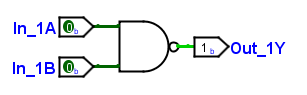
\includegraphics{gfx/50-7400}
	\caption{7424: Single NAND Gate Circuit}
	\label{fig:50-7424}
\end{figure}

The 7424 device in \LE uses the wiring connections indicated in Table \ref{tab:50-7424}.

\begin{table}[H]
	\sffamily
	\newcommand{\head}[1]{\textcolor{white}{\textbf{#1}}}		
	\begin{center}
		\rowcolors{2}{gray!10}{white} % Color every other line a light gray
		\begin{tabular}{rl} 
			\rowcolor{black!75}
			\head{Logisim Label} & \head{Function} \\
			Input: 1   & In 1A  \\
			Input: 2   & In 1B  \\
			Output: 3  & Out 1Y \\
			Input: 4   & In 2A  \\
			Input: 5   & In 2B  \\
			Output: 6  & Out 2Y \\
			Output: 8  & Out 3Y \\
			Input: 9   & In 3A  \\
			Input: 10  & In 3B  \\
			Output: 11 & Out 4Y \\
			Input: 12  & In 4A  \\
			Input: 13  & In 4B  \\
		\end{tabular}
	\end{center}
	\caption{Pinout For 7424}
	\label{tab:50-7424}
\end{table}

\section{7427: Triple 3-Input NOR Gate}

This device contains three independent 3-input NOR gates. Figure \ref{fig:50-7427} is a logic diagram of one of the three circuits.

\begin{figure}[H]
	\centering
	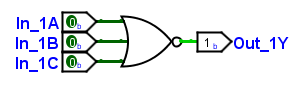
\includegraphics{gfx/50-7427}
	\caption{7411: Single 3-Input NOR Gate Circuit}
	\label{fig:50-7427}
\end{figure}

The 7427 device in \LE uses the wiring connections indicated in Table \ref{tab:50-7427}.

\begin{table}[H]
	\sffamily
	\newcommand{\head}[1]{\textcolor{white}{\textbf{#1}}}		
	\begin{center}
		\rowcolors{2}{gray!10}{white} % Color every other line a light gray
		\begin{tabular}{rl} 
			\rowcolor{black!75}
			\head{Logisim Label} & \head{Function} \\
			Input: 1   & In 1A  \\
			Input: 2   & In 1B  \\
			Input: 3   & In 2A \\
			Input: 4   & In 2B  \\
			Input: 5   & In 2C  \\
			Output: 6  & Out 2Y \\
			Output: 8  & Out 3Y \\
			Input: 9   & In 3A  \\
			Input: 10  & In 3B  \\
			Input: 11  & In 3C \\
			Output: 12 & Out 1Y  \\
			Input: 13  & In 1C  \\
		\end{tabular}
	\end{center}
	\caption{Pinout For 7427}
	\label{tab:50-7427}
\end{table}

\section{7430: Single 8-Input NAND Gate}

This device contains a single 8-input NAND gate. The logic for this gate is $ Y = \overline{A \cdot B \cdot C \cdot D \cdot E \cdot F \cdot G \cdot H} $. Figure \ref{fig:50-7430} is a logic diagram of the circuit.

\begin{figure}[H]
	\centering
	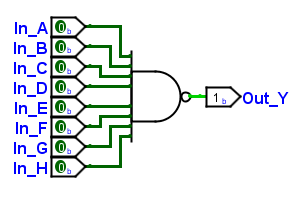
\includegraphics{gfx/50-7430}
	\caption{7430: Single 8-Input NAND Gate}
	\label{fig:50-7430}
\end{figure}

The 7430 device in \LE uses the wiring connections indicated in Table \ref{tab:50-7430}.

\begin{table}[H]
	\sffamily
	\newcommand{\head}[1]{\textcolor{white}{\textbf{#1}}}		
	\begin{center}
		\rowcolors{2}{gray!10}{white} % Color every other line a light gray
		\begin{tabular}{rl} 
			\rowcolor{black!75}
			\head{Logisim Label} & \head{Function} \\
			Input: 1    & In A \\
			Input: 2    & In B \\
			Input: 3    & In C \\
			Input: 4    & In D \\
			Input: 5    & In E \\
			Input: 6    & In F \\
			Output: 8   & Out Y \\
			Pin 9: NC   & Not Connected \\
			Pin 10: NC  & Not Connected \\
			Input: 11   & In G \\
			Input: 12   & In H  \\
			Pin 13: NC  & Not Connected  \\
		\end{tabular}
	\end{center}
	\caption{Pinout For 7430}
	\label{tab:50-7430}
\end{table}

\section{7432: Quad 2-Input OR Gate}

This device contains four independent 2-input OR gates. Figure \ref{fig:50-7432} is a logic diagram of one of the four circuits.

\begin{figure}[H]
	\centering
	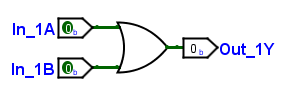
\includegraphics{gfx/50-7432}
	\caption{7432: Single OR Gate Circuit}
	\label{fig:50-7432}
\end{figure}

The 7432 device in \LE uses the wiring connections indicated in Table \ref{tab:50-7432}.

\begin{table}[H]
	\sffamily
	\newcommand{\head}[1]{\textcolor{white}{\textbf{#1}}}		
	\begin{center}
		\rowcolors{2}{gray!10}{white} % Color every other line a light gray
		\begin{tabular}{rl} 
			\rowcolor{black!75}
			\head{Logisim Label} & \head{Function} \\
			Input: 1   & In 1A  \\
			Input: 2   & In 1B  \\
			Output: 3  & Out 1Y \\
			Input: 4   & In 2A  \\
			Input: 5   & In 2B  \\
			Output: 6  & Out 2Y \\
			Output: 8  & Out 3Y \\
			Input: 9   & In 3A  \\
			Input: 10  & In 3B  \\
			Output: 11 & Out 4Y \\
			Input: 12  & In 4A  \\
			Input: 13  & In 4B  \\
		\end{tabular}
	\end{center}
	\caption{Pinout For 7432}
	\label{tab:50-7432}
\end{table}

\section{7436: Quad 2-Input NOR Gate}

This device contains four independent 2-input NOR gates. This device is essentially the same as the 7402. Figure \ref{fig:50-7436} is a logic diagram of one of the four circuits.

\begin{figure}[H]
	\centering
	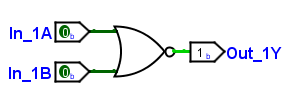
\includegraphics{gfx/50-7402}
	\caption{7436: Single NOR Gate Circuit}
	\label{fig:50-7436}
\end{figure}

The 7436 device in \LE uses the wiring connections indicated in Table \ref{tab:50-7436}.

\begin{table}[H]
	\sffamily
	\newcommand{\head}[1]{\textcolor{white}{\textbf{#1}}}		
	\begin{center}
		\rowcolors{2}{gray!10}{white} % Color every other line a light gray
		\begin{tabular}{rl} 
			\rowcolor{black!75}
			\head{Logisim Label} & \head{Function} \\
			Input: 1   & In 1A  \\
			Input: 2   & In 1B  \\
			Output: 3  & Out 1Y \\
			Input: 4   & In 2A  \\
			Input: 5   & In 2B  \\
			Output: 6  & Out 2Y \\
			Output: 8  & Out 3Y \\
			Input: 9   & In 3A  \\
			Input: 10  & In 3B  \\
			Output: 11 & Out 4Y \\
			Input: 12  & In 4A  \\
			Input: 13  & In 4B  \\
		\end{tabular}
	\end{center}
	\caption{Pinout For 7436}
	\label{tab:50-7436}
\end{table}

\section{7442: BCD to Decimal Decoder}

This device takes a BDC input and deactivates a single line corresponding to the input number. It is often called a ``One-Of-Ten'' decoder. As an example, if $ 0111_{BCD} $ is input then line 7-of-10 will go low while all other outputs will remain high. Figure \ref{fig:50-7442} illustrates a 7442 \ac{IC} in a very simple circuit.

\begin{figure}[H]
	\centering
	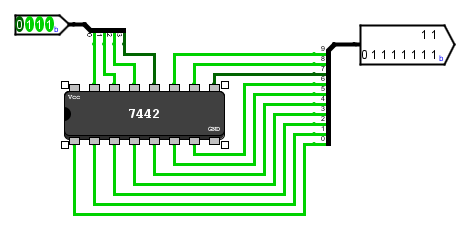
\includegraphics[width=\maxwidth{.95\linewidth}]{gfx/50-7442}
	\caption{7442: BCD to Decimal Decoder}
	\label{fig:50-7442}
\end{figure}

Table \ref{tab:50-7442a} is the truth table for this device. Any BCD input greater than $ 1001 $ is ignored and all outputs will be high for those inputs.

\begin{table}[H]
	\sffamily
	\newcommand{\head}[1]{\textcolor{white}{\textbf{#1}}}		
	\begin{center}
		%\rowcolors{2}{gray!10}{white} % Color every other line light gray - Note: makes the vline vanish
		\begin{tabular}{cccc | cccccccccc} 
			\rowcolor{black!75}
			\multicolumn{4}{c}{\head{Inputs}} & \multicolumn{10}{c}{\head{Output}} \\
			\textbf{A} & \textbf{B} & \textbf{C} & \textbf{D} & \textbf{0} & \textbf{1} & \textbf{2} & \textbf{3} & \textbf{4} & \textbf{5} & \textbf{6} & \textbf{7} & \textbf{8} & \textbf{9} \\
			\hline
			0 & 0 & 0 & 0  & 0 & 1 & 1 & 1 & 1 & 1 & 1 & 1 & 1 & 1 \\
			0 & 0 & 0 & 1  & 1 & 0 & 1 & 1 & 1 & 1 & 1 & 1 & 1 & 1 \\
			0 & 0 & 1 & 0  & 1 & 1 & 0 & 1 & 1 & 1 & 1 & 1 & 1 & 1 \\
			0 & 0 & 1 & 1  & 1 & 1 & 1 & 0 & 1 & 1 & 1 & 1 & 1 & 1 \\
			0 & 1 & 0 & 0  & 1 & 1 & 1 & 1 & 0 & 1 & 1 & 1 & 1 & 1 \\
			0 & 1 & 0 & 1  & 1 & 1 & 1 & 1 & 1 & 0 & 1 & 1 & 1 & 1 \\
			0 & 1 & 1 & 0  & 1 & 1 & 1 & 1 & 1 & 1 & 0 & 1 & 1 & 1 \\
			0 & 1 & 1 & 1  & 1 & 1 & 1 & 1 & 1 & 1 & 1 & 0 & 1 & 1 \\
			1 & 0 & 0 & 0  & 1 & 1 & 1 & 1 & 1 & 1 & 1 & 1 & 0 & 1 \\
			1 & 0 & 0 & 1  & 1 & 1 & 1 & 1 & 1 & 1 & 1 & 1 & 1 & 0 \\
		\end{tabular}
	\end{center}
	\caption{Truth Table For The 7442 Circuit}
	\label{tab:50-7442a}
\end{table}

The 7442 device in \LE uses the wiring connections indicated in Table \ref{tab:50-7442b}.

\begin{table}[H]
	\sffamily
	\newcommand{\head}[1]{\textcolor{white}{\textbf{#1}}}		
	\begin{center}
		\rowcolors{2}{gray!10}{white} % Color every other line a light gray
		\begin{tabular}{rl} 
			\rowcolor{black!75}
			\head{Logisim Label} & \head{Function} \\
			Output 1: O0  & Out 0 \\
			Output 2: O1  & Out 1 \\
			Output 3: O2  & Out 2 \\
			Output 4: O3  & Out 3 \\
			Output 5: O4  & Out 4 \\
			Output 6: O5  & Out 5 \\
			Output 7: O6  & Out 6 \\
			Output 8: O7  & Out 7 \\
			Output 10: O8 & Out 8 \\
			Output 11: O9 & Out 9 \\
			Input 12: D   & In D  \\
			Input 13: C   & In C  \\
			Input 14: B   & In B  \\
			Input 15: A   & In A  \\
		\end{tabular}
	\end{center}
	\caption{Pinout For 7442}
	\label{tab:50-7442b}
\end{table}

\section{7443: Excess-3 to Decimal Decoder}

This device takes an Excess-3 input and deactivates a single line corresponding to the input number. It is often called a ``One-Of-Ten'' decoder. As an example, if $ 0011_{Ex3} $ is input then line 0-of-10 will go low while all other outputs will remain high. This is wired in exactly the same way as the 7442 \ac{IC} illustrated in Figure \ref{fig:50-7442}.

Table \ref{tab:50-7443a} is the truth table for this device. Any input numbers other than those found in the truth table are ignored and all outputs will be high for those inputs.

\begin{table}[H]
	\sffamily
	\newcommand{\head}[1]{\textcolor{white}{\textbf{#1}}}		
	\begin{center}
		%\rowcolors{2}{gray!10}{white} % Color every other line light gray - Note: makes the vline vanish
		\begin{tabular}{cccc | cccccccccc} 
			\rowcolor{black!75}
			\multicolumn{4}{c}{\head{Inputs}} & \multicolumn{10}{c}{\head{Output}} \\
			\textbf{A} & \textbf{B} & \textbf{C} & \textbf{D} & \textbf{0} & \textbf{1} & \textbf{2} & \textbf{3} & \textbf{4} & \textbf{5} & \textbf{6} & \textbf{7} & \textbf{8} & \textbf{9} \\
			\hline
			0 & 0 & 1 & 1  & 0 & 1 & 1 & 1 & 1 & 1 & 1 & 1 & 1 & 1 \\
			0 & 1 & 0 & 0  & 1 & 0 & 1 & 1 & 1 & 1 & 1 & 1 & 1 & 1 \\
			0 & 1 & 0 & 1  & 1 & 1 & 0 & 1 & 1 & 1 & 1 & 1 & 1 & 1 \\
			0 & 1 & 1 & 0  & 1 & 1 & 1 & 0 & 1 & 1 & 1 & 1 & 1 & 1 \\
			0 & 1 & 1 & 1  & 1 & 1 & 1 & 1 & 0 & 1 & 1 & 1 & 1 & 1 \\
			1 & 0 & 0 & 0  & 1 & 1 & 1 & 1 & 1 & 0 & 1 & 1 & 1 & 1 \\
			1 & 0 & 0 & 1  & 1 & 1 & 1 & 1 & 1 & 1 & 0 & 1 & 1 & 1 \\
			1 & 0 & 1 & 0  & 1 & 1 & 1 & 1 & 1 & 1 & 1 & 0 & 1 & 1 \\
			1 & 0 & 1 & 1  & 1 & 1 & 1 & 1 & 1 & 1 & 1 & 1 & 0 & 1 \\
			1 & 1 & 0 & 0  & 1 & 1 & 1 & 1 & 1 & 1 & 1 & 1 & 1 & 0 \\
		\end{tabular}
	\end{center}
	\caption{Truth Table For The 7443 Circuit}
	\label{tab:50-7443a}
\end{table}

The 7443 device in \LE uses the wiring connections indicated in Table \ref{tab:50-7443b}.

\begin{table}[H]
	\sffamily
	\newcommand{\head}[1]{\textcolor{white}{\textbf{#1}}}		
	\begin{center}
		\rowcolors{2}{gray!10}{white} % Color every other line a light gray
		\begin{tabular}{rl} 
			\rowcolor{black!75}
			\head{Logisim Label} & \head{Function} \\
			Output 1: O0  & Out 0 \\
			Output 2: O1  & Out 1 \\
			Output 3: O2  & Out 2 \\
			Output 4: O3  & Out 3 \\
			Output 5: O4  & Out 4 \\
			Output 6: O5  & Out 5 \\
			Output 7: O6  & Out 6 \\
			Output 8: O7  & Out 7 \\
			Output 10: O8 & Out 8 \\
			Output 11: O9 & Out 9 \\
			Input 12: D   & In D  \\
			Input 13: C   & In C  \\
			Input 14: B   & In B  \\
			Input 15: A   & In A  \\
		\end{tabular}
	\end{center}
	\caption{Pinout For 7443}
	\label{tab:50-7443b}
\end{table}

\section{7444: Gray to Decimal Decoder}

This device takes a Gray Excess Code, which is a combination of Gray and Excess-3 Codes, input and deactivates a single line corresponding to the input number. It is often called a ``One-Of-Ten'' decoder. As an example, if $ 1100_{GrayEx3} $ is input then line 5-of-10 will go low while all other outputs will remain high. This is wired in exactly the same way as the 7442 \ac{IC} illustrated in Figure \ref{fig:50-7442}.

Table \ref{tab:50-7444a} is the truth table for this device. Any input numbers other than those found in the truth table are ignored and all outputs will be high for those inputs.

\begin{table}[H]
	\sffamily
	\newcommand{\head}[1]{\textcolor{white}{\textbf{#1}}}		
	\begin{center}
		%\rowcolors{2}{gray!10}{white} % Color every other line light gray - Note: makes the vline vanish
		\begin{tabular}{cccc | cccccccccc} 
			\rowcolor{black!75}
			\multicolumn{4}{c}{\head{Inputs}} & \multicolumn{10}{c}{\head{Output}} \\
			\textbf{A} & \textbf{B} & \textbf{C} & \textbf{D} & \textbf{0} & \textbf{1} & \textbf{2} & \textbf{3} & \textbf{4} & \textbf{5} & \textbf{6} & \textbf{7} & \textbf{8} & \textbf{9} \\
			\hline
			0 & 0 & 1 & 0  & 0 & 1 & 1 & 1 & 1 & 1 & 1 & 1 & 1 & 1 \\
			0 & 1 & 1 & 0  & 1 & 0 & 1 & 1 & 1 & 1 & 1 & 1 & 1 & 1 \\
			0 & 1 & 1 & 1  & 1 & 1 & 0 & 1 & 1 & 1 & 1 & 1 & 1 & 1 \\
			0 & 1 & 0 & 1  & 1 & 1 & 1 & 0 & 1 & 1 & 1 & 1 & 1 & 1 \\
			0 & 1 & 0 & 0  & 1 & 1 & 1 & 1 & 0 & 1 & 1 & 1 & 1 & 1 \\
			1 & 1 & 0 & 0  & 1 & 1 & 1 & 1 & 1 & 0 & 1 & 1 & 1 & 1 \\
			1 & 1 & 0 & 1  & 1 & 1 & 1 & 1 & 1 & 1 & 0 & 1 & 1 & 1 \\
			1 & 1 & 1 & 1  & 1 & 1 & 1 & 1 & 1 & 1 & 1 & 0 & 1 & 1 \\
			1 & 1 & 1 & 0  & 1 & 1 & 1 & 1 & 1 & 1 & 1 & 1 & 0 & 1 \\
			1 & 0 & 1 & 0  & 1 & 1 & 1 & 1 & 1 & 1 & 1 & 1 & 1 & 0 \\
		\end{tabular}
	\end{center}
	\caption{Truth Table For The 7444 Circuit}
	\label{tab:50-7444a}
\end{table}

The 7443 device in \LE uses the wiring connections indicated in Table \ref{tab:50-7444b}.

\begin{table}[H]
	\sffamily
	\newcommand{\head}[1]{\textcolor{white}{\textbf{#1}}}		
	\begin{center}
		\rowcolors{2}{gray!10}{white} % Color every other line a light gray
		\begin{tabular}{rl} 
			\rowcolor{black!75}
			\head{Logisim Label} & \head{Function} \\
			Output 1: O0  & Out 0 \\
			Output 2: O1  & Out 1 \\
			Output 3: O2  & Out 2 \\
			Output 4: O3  & Out 3 \\
			Output 5: O4  & Out 4 \\
			Output 6: O5  & Out 5 \\
			Output 7: O6  & Out 6 \\
			Output 8: O7  & Out 7 \\
			Output 10: O8 & Out 8 \\
			Output 11: O9 & Out 9 \\
			Input 12: D   & In D  \\
			Input 13: C   & In C  \\
			Input 14: B   & In B  \\
			Input 15: A   & In A  \\
		\end{tabular}
	\end{center}
	\caption{Pinout For 7444}
	\label{tab:50-7444b}
\end{table}

\section{7447: BCD to 7-Segment Decoder}

This device takes a BCD Code input and activates a combination of outputs such that a 7-segment display will correctly indicate the input number. Figure \ref{fig:50-7447} illustrates a 7447 \ac{IC} in a very simple circuit.

\begin{figure}[H]
	\centering
	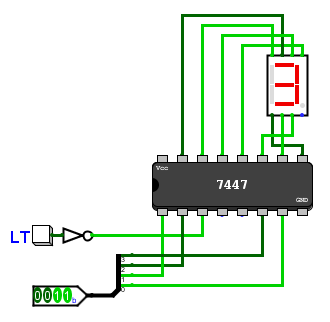
\includegraphics{gfx/50-7447}
	\caption{7447: BCD to 7-Segment Decoder}
	\label{fig:50-7447}
\end{figure}

Table \ref{tab:50-7447} is the truth table for this device. 

\begin{table}[H]
	\sffamily
	\newcommand{\head}[1]{\textcolor{white}{\textbf{#1}}}		
	\begin{center}
		%\rowcolors{2}{gray!10}{white} % Color every other line light gray - Note: makes the vline vanish
		\begin{tabular}{cccc | ccccccc} 
			\rowcolor{black!75}
			\multicolumn{4}{c}{\head{Inputs}} & \multicolumn{7}{c}{\head{Output}} \\
			\textbf{A} & \textbf{B} & \textbf{C} & \textbf{D} & \textbf{a} & \textbf{b} & \textbf{c} & \textbf{d} & \textbf{e} & \textbf{f} & \textbf{g} \\
			\hline
			0 & 0 & 0 & 0  & 1 & 1 & 1 & 1 & 1 & 1 & 0 \\
			0 & 0 & 0 & 1  & 0 & 1 & 1 & 0 & 0 & 0 & 0 \\
			0 & 0 & 1 & 0  & 1 & 1 & 0 & 1 & 1 & 0 & 1 \\
			0 & 0 & 1 & 1  & 1 & 1 & 1 & 1 & 0 & 0 & 1 \\
			0 & 1 & 0 & 0  & 0 & 1 & 1 & 0 & 0 & 1 & 1 \\
			0 & 1 & 0 & 1  & 1 & 0 & 1 & 1 & 0 & 1 & 1 \\
			0 & 1 & 1 & 0  & 1 & 0 & 1 & 1 & 1 & 1 & 1 \\
			0 & 1 & 1 & 1  & 1 & 1 & 1 & 0 & 0 & 0 & 0 \\
			1 & 0 & 0 & 0  & 1 & 1 & 1 & 1 & 1 & 1 & 1 \\
			1 & 0 & 0 & 1  & 1 & 1 & 1 & 0 & 0 & 1 & 1 \\
			1 & 0 & 1 & 0  & 1 & 1 & 1 & 0 & 1 & 1 & 1 \\
			1 & 0 & 1 & 1  & 0 & 0 & 1 & 1 & 1 & 1 & 1 \\
			1 & 1 & 0 & 0  & 1 & 0 & 0 & 1 & 1 & 1 & 0 \\
			1 & 1 & 0 & 1  & 0 & 1 & 1 & 1 & 1 & 0 & 1 \\
			1 & 1 & 1 & 0  & 1 & 0 & 0 & 1 & 1 & 1 & 1 \\
			1 & 1 & 1 & 1  & 1 & 0 & 0 & 0 & 1 & 1 & 1 \\
		\end{tabular}
	\end{center}
	\caption{Truth Table For The 7447 Circuit}
	\label{tab:50-7447}
\end{table}

The 7447 device in \LE uses the wiring connections indicated in Table \ref{tab:50-7447a}.

\begin{table}[H]
	\sffamily
	\newcommand{\head}[1]{\textcolor{white}{\textbf{#1}}}		
	\begin{center}
		\rowcolors{2}{gray!10}{white} % Color every other line a light gray
		\begin{tabular}{rl} 
			\rowcolor{black!75}
			\head{Logisim Label} & \head{Function} \\
			Input 1: B   & B   \\
			Input 2: C   & C   \\
			Input 3: LT  & LT  \\
			Input 4: BI  & BI  \\
			Input 5: RBI & RBI \\
			Input 6: D   & D   \\
			Input 7: A   & A   \\
			Output 8: e  & e   \\
			Output 10: d & d   \\
			Output 11: c & c   \\
			Output 12: b & b   \\
			Output 13: a & a   \\
			Output 14: g & g   \\
			Output 15: f & f   \\
		\end{tabular}
	\end{center}
	\caption{Pinout For 7447}
	\label{tab:50-7447a}
\end{table}

\section{7451: Dual AND-OR-INVERT Gate}

This device contains two independent AND-OR-INVERT gates. Figure \ref{fig:50-7451} is a logic diagram of one of the two circuits.

\begin{figure}[H]
	\centering
	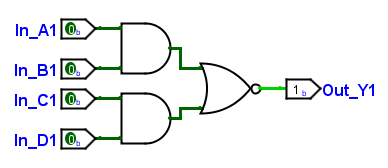
\includegraphics{gfx/50-7451}
	\caption{7451: Single AND-OR-INVERT Gate Circuit}
	\label{fig:50-7451}
\end{figure}

The 7451 device in \LE uses the wiring connections indicated in Table \ref{tab:50-7451}.

\begin{table}[H]
	\sffamily
	\newcommand{\head}[1]{\textcolor{white}{\textbf{#1}}}		
	\begin{center}
		\rowcolors{2}{gray!10}{white} % Color every other line a light gray
		\begin{tabular}{rl} 
			\rowcolor{black!75}
			\head{Logisim Label} & \head{Function} \\
			Input 1: A1   & In A1         \\
			Input 2: A2   & In A2         \\
			Input 3: B2   & In B2         \\
			Input 4: C2   & In C2         \\
			Input 5: D2   & In D2         \\
			Output 6: Y2  & Out Y2        \\
			Output 8: Y1  & Out Y1        \\
			Input 9: C1   & In C1         \\
			Input 10: D1  & In D1         \\
			Pin 11: NC    & Not Connected \\
			Pin 12: NC    & Not Connected \\
			Input 13: B1  & In B1         \\
		\end{tabular}
	\end{center}
	\caption{Pinout For 7451}
	\label{tab:50-7451}
\end{table}

\section{7454: Four Wide AND-OR-INVERT Gate}

This device contains a single four-wide AND-OR-INVERT gate. Figure \ref{fig:50-7454} is a logic diagram of the circuit.

\begin{figure}[H]
	\centering
	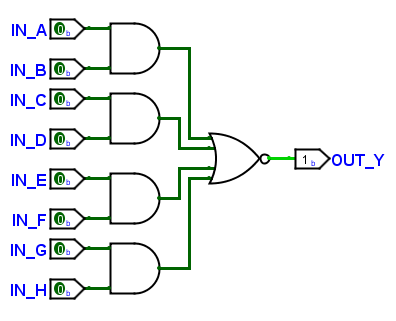
\includegraphics{gfx/50-7454}
	\caption{7454: Four Wide AND-OR-INVERT Gate Circuit}
	\label{fig:50-7454}
\end{figure}

The 7454 device in \LE uses the wiring connections indicated in Table \ref{tab:50-7454}.

\begin{table}[H]
	\sffamily
	\newcommand{\head}[1]{\textcolor{white}{\textbf{#1}}}		
	\begin{center}
		\rowcolors{2}{gray!10}{white} % Color every other line a light gray
		\begin{tabular}{rl} 
			\rowcolor{black!75}
			\head{Logisim Label} & \head{Function} \\
			Input 1: A   & In A          \\
			Input 2: C   & In C          \\
			Input 3: D   & In D          \\
			Input 4: E   & In E          \\
			Input 5: F   & In F          \\
			Pin 6: NC    & Not Connected \\
			Output 8: Y  & Out Y         \\
			Input 9: G   & In G          \\
			Input 10: H  & In H          \\
			Pin 11: NC   & Not Connected \\
			Pin 12: NC   & Not Connected \\
			Input 13: B  & In B          \\
		\end{tabular}
	\end{center}
	\caption{Pinout For 7454}
	\label{tab:50-7454}
\end{table}

\section{7458: Dual AND-OR Gate}

This device contains a two AND-OR gates. One has three-input AND gates and the other has two-input AND gates. Figure \ref{fig:50-7458} is a logic diagram of the circuit.

\begin{figure}[H]
	\centering
	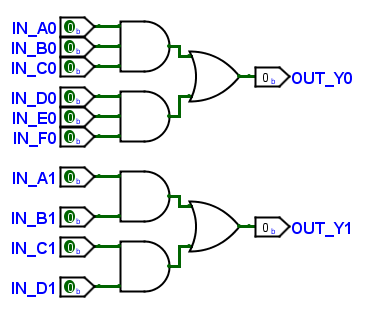
\includegraphics{gfx/50-7458}
	\caption{7458: Dual AND-OR Gate Circuit}
	\label{fig:50-7458}
\end{figure}

The 7458 device in \LE uses the wiring connections indicated in Table \ref{tab:50-7458}.

\begin{table}[H]
	\sffamily
	\newcommand{\head}[1]{\textcolor{white}{\textbf{#1}}}		
	\begin{center}
		\rowcolors{2}{gray!10}{white} % Color every other line a light gray
		\begin{tabular}{rl} 
			\rowcolor{black!75}
			\head{Logisim Label} & \head{Function} \\
			Input 1: A0   & In A0  \\
			Input 2: A1   & In A1  \\
			Input 3: B1   & In B1  \\
			Input 4: C1   & In C1  \\
			Input 5: D1   & In D1  \\
			Output 6: Y1  & Out Y1 \\
			Output 8: Y0  & Out Y0 \\
			Input 9: D0   & In D0  \\
			Input 10: E0  & In E0 \\
			Input 11: F0  & In F0 \\
			Input 12: B0  & In B0 \\
			Input 13: C0  & In C0 \\
		\end{tabular}
	\end{center}
	\caption{Pinout For 7458}
	\label{tab:50-7458}
\end{table}

\section{7464: 4-2-3-2 AND-OR-INVERT Gate}

This device contains four AND gates of different input sizes that feed a NOR gate. Figure \ref{fig:50-7464} is a logic diagram of the circuit.

\begin{figure}[H]
	\centering
	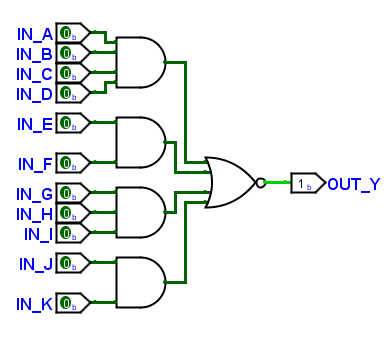
\includegraphics{gfx/50-7464}
	\caption{7464: 4-2-3-2 AND-OR-INVERT Gate Circuit}
	\label{fig:50-7464}
\end{figure}

The 7464 device in \LE uses the wiring connections indicated in Table \ref{tab:50-7464}.

\begin{table}[H]
	\sffamily
	\newcommand{\head}[1]{\textcolor{white}{\textbf{#1}}}		
	\begin{center}
		\rowcolors{2}{gray!10}{white} % Color every other line a light gray
		\begin{tabular}{rl} 
			\rowcolor{black!75}
			\head{Logisim Label} & \head{Function} \\
			Input 1: A   & In A  \\
			Input 2: E   & In E  \\
			Input 3: F   & In F  \\
			Input 4: G   & In G  \\
			Input 5: H   & In H  \\
			Input 6: I   & In I  \\
			Output 8: Y  & Out Y \\
			Input 9: J   & In J  \\
			Input 10: K  & In K  \\
			Input 11: B  & In B  \\
			Input 12: C  & In C  \\
			Input 13: D  & In D  \\
		\end{tabular}
	\end{center}
	\caption{Pinout For 7464}
	\label{tab:50-7464}
\end{table}

\section{7474: Dual D-Flipflops with Preset and Clear}

This device contains two D-Flipflops, each with its own preset and clear. The 7474 device in \LE uses the wiring connections indicated in Table \ref{tab:50-7474}.

\begin{table}[H]
	\sffamily
	\newcommand{\head}[1]{\textcolor{white}{\textbf{#1}}}		
	\begin{center}
		\rowcolors{2}{gray!10}{white} % Color every other line a light gray
		\begin{tabular}{rl} 
			\rowcolor{black!75}
			\head{Logisim Label} & \head{Function} \\
			Input 1: nCLR1  & On low, clear FF1 \\
			Input 2: D1     & FF1 data input    \\
			Input 3: CLK1   & FF1 clock         \\
			Input 4: nPRE1  & On low, set FF1   \\
			Output 5: Q1    & FF1 Q-out         \\
			Output 6: nQ1   & FF1 Q-not-out     \\
			Output 8: nQ2   & FF2 Q-not-out     \\
			Output 9: Q2    & FF2 Q-out         \\
			Input 10: nPRE2 & On low, set FF2   \\
			Input 11: CLK2  & FF2 clock         \\
			Input 12: D2    & FF2 data input    \\
			Input 13: nCLR2 & On low, clear FF2 \\
		\end{tabular}
	\end{center}
	\caption{Pinout For 7474}
	\label{tab:50-7474}
\end{table}

\section{7485: 4-Bit Magnitude Comparator}

This device compares two 4-bit numbers and outputs one of three values: $ A>B $, $ A=B $, or $ A<B $. It is also designed to be cascaded by including an input port for each of the three values. The 7485 device in \LE uses the wiring connections indicated in Table \ref{tab:50-7485}.

\begin{table}[H]
	\sffamily
	\newcommand{\head}[1]{\textcolor{white}{\textbf{#1}}}		
	\begin{center}
		\rowcolors{2}{gray!10}{white} % Color every other line a light gray
		\begin{tabular}{rl} 
			\rowcolor{black!75}
			\head{Logisim Label} & \head{Function} \\
			Input 1: B3   & Bit B3                 \\
			Input 2: A<B  & Value from prior stage \\
			Input 3: A=B  & Value from prior stage \\
			Input 4: A>B  & Value from prior stage \\
			Output 5: A>B & High if A>B            \\
			Output 6: A=B & High if A=B            \\
			Output 7: A<B & High if A<B            \\
			Input 9: B0   & Bit B0                 \\
			Input 10: A0  & Bit A0                 \\
			Input 11: B1  & Bit B1                 \\
			Input 12: A1  & Bit A1                 \\
			Input 13: A2  & Bit A2                 \\
			Input 14: B2  & Bit B2                 \\
			Input 15: A3  & Bit A3                 \\
		\end{tabular}
	\end{center}
	\caption{Pinout For 7485}
	\label{tab:50-7485}
\end{table}

\section{7486: Quad 2-Input XOR Gate}

This device contains four independent 2-input XOR gates. Figure \ref{fig:50-7486} is a logic diagram of one of the four circuits.

\begin{figure}[H]
	\centering
	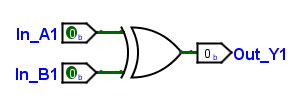
\includegraphics{gfx/50-7486}
	\caption{7486: Single XOR Gate Circuit}
	\label{fig:50-7486}
\end{figure}

The 7486 device in \LE uses the wiring connections indicated in Table \ref{tab:50-7486}.

\begin{table}[H]
	\sffamily
	\newcommand{\head}[1]{\textcolor{white}{\textbf{#1}}}		
	\begin{center}
		\rowcolors{2}{gray!10}{white} % Color every other line a light gray
		\begin{tabular}{rl} 
			\rowcolor{black!75}
			\head{Logisim Label} & \head{Function} \\
			Input: 1   & In 1A  \\
			Input: 2   & In 1B  \\
			Output: 3  & Out 1Y \\
			Input: 4   & In 2A  \\
			Input: 5   & In 2B  \\
			Output: 6  & Out 2Y \\
			Output: 8  & Out 3Y \\
			Input: 9   & In 3A  \\
			Input: 10  & In 3B  \\
			Output: 11 & Out 4Y \\
			Input: 12  & In 4A  \\
			Input: 13  & In 4B  \\
		\end{tabular}
	\end{center}
	\caption{Pinout For 7486}
	\label{tab:50-7486}
\end{table}

\section{74125: Quad Bus Buffer, 3-State Gate}

This device contains four independent buffers. When each is enabled with a low on the enable line then the input is passed to the output, when not enabled then the output floats. Figure \ref{fig:50-74125} is a logic diagram of one of the four circuits.

\begin{figure}[H]
	\centering
	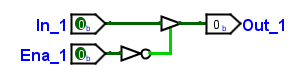
\includegraphics{gfx/50-74125}
	\caption{74125: Single Buffer Circuit}
	\label{fig:50-74125}
\end{figure}

The 74125 device in \LE uses the wiring connections indicated in Table \ref{tab:50-74125}.

\begin{table}[H]
	\sffamily
	\newcommand{\head}[1]{\textcolor{white}{\textbf{#1}}}		
	\begin{center}
		\rowcolors{2}{gray!10}{white} % Color every other line a light gray
		\begin{tabular}{rl} 
			\rowcolor{black!75}
			\head{Logisim Label} & \head{Function} \\
			Input: 1   & nEna 1 \\
			Input: 2   & In 1  \\
			Output: 3  & Out 1 \\
			Input: 4   & nEna 2 \\
			Input: 5   & In 2  \\
			Output: 6  & Out 2 \\
			Output: 8  & Out 3 \\
			Input: 9   & In 3  \\
			Input: 10  & nEna 3 \\
			Output: 11 & Out 4 \\
			Input: 12  & In 4  \\
			Input: 13  & nEna 4 \\
		\end{tabular}
	\end{center}
	\caption{Pinout For 74125}
	\label{tab:50-74125}
\end{table}

\section{74165: 8-Bit Parallel-to-Serial Shift Register}

This device can accept data in either parallel or serial form and shift it out in serial form. The 74165 device in \LE uses the wiring connections indicated in Table \ref{tab:50-74165}.

\begin{table}[H]
	\sffamily
	\newcommand{\head}[1]{\textcolor{white}{\textbf{#1}}}		
	\begin{center}
		\rowcolors{2}{gray!10}{white} % Color every other line a light gray
		\begin{tabular}{rl} 
			\rowcolor{black!75}
			\head{Logisim Label} & \head{Function} \\
			Input 1: Shift/Load     & Load when low, shift when high \\
			Input 2: Clock          & Clock                          \\
			Input 3: P4             & Input bit 4                    \\
			Input 4: P5             & Input bit 5                    \\
			Input 5: P6             & Input bit 6                    \\
			Input 6: P7             & Input bit 7                    \\
			Output 7: Q7n           & Complement of serial out       \\
			Output 9: Q7            & Serial out                     \\
			Input 10: Serial Input  & Serial data in                 \\
			Input 11: P0            & Input bit 0                    \\
			Input 12: P1            & Input bit 1                    \\
			Input 13: P2            & Input bit 2                    \\
			Input 14: P3            & Input bit 3                    \\
			Input 15: Clock Inhibit & Clock inhibit                  \\
		\end{tabular}
	\end{center}
	\caption{Pinout For 74165}
	\label{tab:50-74165}
\end{table}


\section{74175: Quad D-Flipflops with Sync Reset}

This device contains four D-Flipflops with a single clock and master reset. The 74175 device in \LE uses the wiring connections indicated in Table \ref{tab:50-74175}.

\begin{table}[H]
	\sffamily
	\newcommand{\head}[1]{\textcolor{white}{\textbf{#1}}}		
	\begin{center}
		\rowcolors{2}{gray!10}{white} % Color every other line a light gray
		\begin{tabular}{rl} 
			\rowcolor{black!75}
			\head{Logisim Label} & \head{Function} \\
			Input 1: nCLR  & On low, clear all FF \\
			Output 2: Q1   & FF1 Q-out            \\
			Output 3: nQ1  & FF1 Q-not-out        \\
			Input 4: D1    & FF1 data input       \\
			Input 5: D2    & FF2 data input       \\
			Output 6: nQ2  & FF2 Q-not-out        \\
			Output 7: Q2   & FF2 Q-out            \\
			Input 9: CLK   & Clock for all FF     \\
			Output 10: Q3  & FF3 Q-out            \\
			Output 11: nQ3 & FF3 Q-not-out        \\
			Input 12: D3   & FF3 data input       \\
			Input 13: D4   & FF4 data input       \\
			Output 14: nQ4 & FF4 Q-not-out        \\
			Output 15: Q4  & FF4 Q-out            \\
		\end{tabular}
	\end{center}
	\caption{Pinout For 74175}
	\label{tab:50-74175}
\end{table}

\section{74266: Quad 2-Input XNOR Gate}

This device contains four independent 2-input XNOR gates. Figure \ref{fig:50-74266} is a logic diagram of one of the four circuits.

\begin{figure}[H]
	\centering
	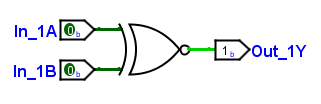
\includegraphics{gfx/50-74266}
	\caption{74266: Single XNOR Gate Circuit}
	\label{fig:50-74266}
\end{figure}

The 74266 device in \LE uses the wiring connections indicated in Table \ref{tab:50-74266}.

\begin{table}[H]
	\sffamily
	\newcommand{\head}[1]{\textcolor{white}{\textbf{#1}}}		
	\begin{center}
		\rowcolors{2}{gray!10}{white} % Color every other line a light gray
		\begin{tabular}{rl} 
			\rowcolor{black!75}
			\head{Logisim Label} & \head{Function} \\
			Input: 1   & In 1A  \\
			Input: 2   & In 1B  \\
			Output: 3  & Out 1Y \\
			Input: 4   & In 2A  \\
			Input: 5   & In 2B  \\
			Output: 6  & Out 2Y \\
			Output: 8  & Out 3Y \\
			Input: 9   & In 3A  \\
			Input: 10  & In 3B  \\
			Output: 11 & Out 4Y \\
			Input: 12  & In 4A  \\
			Input: 13  & In 4B  \\
		\end{tabular}
	\end{center}
	\caption{Pinout For 74266}
	\label{tab:50-74266}
\end{table}

\section{74273: Octal D-Flipflop with Clear}

This device contains a single 8-bit D-Flipflop with a single clock and master clear. The 74273 device in \LE uses the wiring connections indicated in Table \ref{tab:50-74273}.

\begin{table}[H]
	\sffamily
	\newcommand{\head}[1]{\textcolor{white}{\textbf{#1}}}		
	\begin{center}
		\rowcolors{2}{gray!10}{white} % Color every other line a light gray
		\begin{tabular}{rl} 
			\rowcolor{black!75}
			\head{Logisim Label} & \head{Function} \\
			Input 1: nCLR & On low, clear the FF \\
			Output 2: Q1  & data bit 1 output    \\
			Input 3: D1   & data bit 1 input     \\
			Input 4: D2   & data bit 2 input     \\
			Output 5: Q2  & data bit 2 output    \\
			Output 6: Q3  & data bit 3 output    \\
			Input 7: D3   & data bit 3 input     \\
			Input 8: D4   & data bit 4 input     \\
			Output 9: Q4  & data bit 4 output    \\
			Input 11: CLK & Clock                \\
			Output 12: Q5 & data bit 5 output    \\
			Input 13: D5  & data bit 5 input     \\
			Input 14: D6  & data bit 6 input     \\
			Output 15: Q6 & data bit 6 output    \\
			Output 16: Q7 & data bit 7 output    \\
			Input 17: D7  & data bit 7 input     \\
			Input 18: D8  & data bit 8 input     \\
			Output 19: Q8 & data bit 8 output    \\
		\end{tabular}
	\end{center}
	\caption{Pinout For 74273}
	\label{tab:50-74273}
\end{table}

\section{74283: 4-Bit Binary Full Adder}

This device contains a 4-bit adder with carry-in and carry-out bits. The 74283 device in \LE uses the wiring connections indicated in Table \ref{tab:50-74283}.

\begin{table}[H]
	\sffamily
	\newcommand{\head}[1]{\textcolor{white}{\textbf{#1}}}		
	\begin{center}
		\rowcolors{2}{gray!10}{white} % Color every other line a light gray
		\begin{tabular}{rl} 
			\rowcolor{black!75}
			\head{Logisim Label} & \head{Function}  \\
			Output 1: $ \sum $2  & Sum, bit 2       \\
			Input 2: B2          & Operand B, bit 2 \\
			Input 3: A2          & Operand A, bit 2 \\
			Output 4: $ \sum $1  & Sum, bit 1       \\
			Input 5: A1          & Operand A, bit 1 \\
			Input 6: B1          & Operand B, bit 1 \\
			Input 7: CIN         & Carry in bit     \\
			Output 9: C4         & Carry out bit    \\
			Output 10: $ \sum $4 & Sum, bit 4       \\
			Input 11: B4         & Operand B, bit 4 \\
			Input 12: A4         & Operand A, bit 4 \\
			Output 13: $ \sum $3 & Sum, bit 3       \\
			Input 14: A3         & Operand A, bit 3 \\
			Input 15: B3         & Operand B, bit 3 \\
		\end{tabular}
	\end{center}
	\caption{Pinout For 74283}
	\label{tab:50-74283}
\end{table}

\section{74377: Octal D-Flipflop with Enable}

This device contains a single 8-bit D-Flipflop with a single clock and enable. The 74377 device in \LE uses the wiring connections indicated in Table \ref{tab:50-74377}.

\begin{table}[H]
	\sffamily
	\newcommand{\head}[1]{\textcolor{white}{\textbf{#1}}}		
	\begin{center}
		\rowcolors{2}{gray!10}{white} % Color every other line a light gray
		\begin{tabular}{rl} 
			\rowcolor{black!75}
			\head{Logisim Label} & \head{Function} \\
			Input 1: nCLKen & On low, enable the clock \\
			Output 2: Q1    & data bit 1 output    \\
			Input 3: D1     & data bit 1 input     \\
			Input 4: D2     & data bit 2 input     \\
			Output 5: Q2    & data bit 2 output    \\
			Output 6: Q3    & data bit 3 output    \\
			Input 7: D3     & data bit 3 input     \\
			Input 8: D4     & data bit 4 input     \\
			Output 9: Q4    & data bit 4 output    \\
			Input 11: CLK   & Clock                \\
			Output 12: Q5   & data bit 5 output    \\
			Input 13: D5    & data bit 5 input     \\
			Input 14: D6    & data bit 6 input     \\
			Output 15: Q6   & data bit 6 output    \\
			Output 16: Q7   & data bit 7 output    \\
			Input 17: D7    & data bit 7 input     \\
			Input 18: D8    & data bit 8 input     \\
			Output 19: Q8   & data bit 8 output    \\
		\end{tabular}
	\end{center}
	\caption{Pinout For 74377}
	\label{tab:50-74377}
\end{table}


%*******************************************************
% New Appendix Here
%*******************************************************
%\chapter{New Appendix Here}
%\label{ap:ch:new_appendix_here}
